%! Author = Philipp Emmenegger
%! Date = 14/07/2021

\section{Interactive Programming}
\textbf{The Problem:}
\begin{itemize}
    \item Haskell programs are pure mathematical functions:
    \begin{itemize}
        \item \textbf{Haskell programs have no side effects}
    \end{itemize}
    \item Reading from the keyboard and writing to the screen are side effects
    \begin{itemize}
        \item \textbf{Interactive programs have side effects}
    \end{itemize}
\end{itemize}
\textbf{The Solution:}\\ 
Interactive programs can be written in Haskell by using \textit{types} to distinguish \textit{pure expressions} from \textit{impure actions} (aka. commands) that may involve side effects.\\ 
\begin{center}
    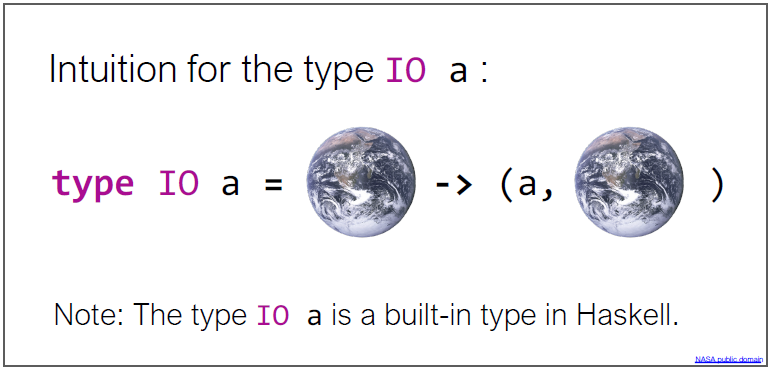
\includegraphics[width=0.6\linewidth]{img/io_type.png}
\end{center}
\begin{itemize}
    \item \textbf{IO Char:} The type of actions that return a character
    \item \textbf{IO ():} The type of purely side effecting actions that return no result value
    \begin{itemize}
        \item (): Type of tuples with no value (unit type), like \textit{void}
    \end{itemize}
\end{itemize}

\subsection{Basic Actions}
\begin{lstlisting}
getChar :: IO Char
\end{lstlisting}
Reads a character from the keyboard, echoes it to the screen and returns the character as its result value.
\begin{lstlisting}
putChar :: Char -> IO ()
\end{lstlisting}
Writes the character \textbf{c} to the screen and returns no result value.
\begin{lstlisting}
return :: a -> IO a
\end{lstlisting}
Returns the value \textbf{v} without performing any interaction.

\subsection{Sequencing}
A sequence of actions can be combined as a single composite action using the keyword \textbf{do}:
\begin{lstlisting}
act :: IO (Char, Char)
act = do {
    x <- getChar;
    getChar;
    y <- getChar;
    return (x, y)
}
\end{lstlisting}
\textbf{Reading a string from the keyboard:}
\begin{lstlisting}
getLine:: IO String 
getLine = do {
    x <- getChar
    if x == '\n' 
        then
            return []
    else
        do {
            xs <- getLine 
            return (x : xs)
        }
}
\end{lstlisting}
\textbf{Writing a string to the screen:}
\begin{lstlisting}
putStr :: String -> IO ()
putStr [] = return ()
putStr (x : xs) = do putChar x
                    putStr xs
\end{lstlisting}
\textbf{Writing a string and moving to a new line}
\begin{lstlisting}
putStrLn :: String -> IO ()
putStrLn xs = do putStr xs
                putChar '\n'
\end{lstlisting}